\documentclass[12pt]{article}
\usepackage{sbc-template}
\usepackage{url}
\usepackage{graphicx}
\usepackage[utf8]{inputenc}
\usepackage{comment}
\usepackage{scalefnt}
%\usepackage[brazilian]{babel}

\sloppy

\title{Técnicas de usabilidade em projetos ágeis aplicadas no desenvolvimento de software livre}

\author{Renan Costa Filgueiras, Paulo Meirelles}
\address{Faculdade Gama – Universidade de Brasília (UnB) – Brasília – DF – Brazil
\email{renan2727@outlook.com, paulormm@unb.br}
}

\usepackage{xcolor}
\newcommand{\TODO}[1]{
  {
    \color{red}\textbf{{#1} (TODO)}
  }
}

\begin{document}

\maketitle
%-------------------------------------------------------------------------------
\begin{abstract}
Many free software projects have no practices to improve usability in their development process, which may influences on the adoption of them.
%
The free software production can be considered an agile methodology from the software engineering point of view.
%
The aim of this study was to investigate what agile usability techniques are addressed by communities agile and software free.
%
For this, we used the technique of systematic review were identified techniques aimed at writing stories, the design of the user, or even the use of beta testing for payment.

\end{abstract}
%-------------------------------------------------------------------------------

%-------------------------------------------------------------------------------
\begin{resumo}
Muitos dos projetos de software livre não possuem práticas para melhoria da usabilidade em seu processo de desenvolvimento, o que pode influenciar na adoção.
%
O desenvolvimento de software livre pode ser considerado um método ágil do ponto de vista da engenharia de software.
%
O objetivo deste trabalho foi investigar quais técnicas de usabilidades ágeis são abordadas pelas comunidades de software livre.
%
Para isso, foi empregada a técnica de revisão sistemática e foram identificadas técnicas voltadas à escrita de histórias, ao design do usuário, ou mesmo o emprego de teste beta por pagamento.

\end{resumo}
%-------------------------------------------------------------------------------

\section{Introdução}
\label{introducao}
%~\cite{martin2008}.
Ao lado da própria dificuldade em se mensurar objetivamente a usabilidade de um sistema, é comum em programas de software livre que haja pouco incentivo (ou interesse) nesse aspecto, dado que a prioridade do mesmo é a implementação das funcionalidades. Essa cultura leva o desenvolvedor a iniciar o projeto pelo código, deixando o design de interfaces em segundo plano~\cite{} %[Thomas 2008].
%

Métodos de usabilidade são utilizados por empresas especialistas em projeto de interação e, nos processos de desenvolvimento de projetos de software fechado, o que garante, em geral, uma melhor usabilidade quando comparados à maioria dos sistemas de software livre.
%

Esse cenário é um dos fatores que limita a expansão de uso e aceitação de sistemas livres, que com baixa usabilidade, perde-se também em confiança dos usuários. O uso desse tipo de sistema limita-se a usuários mais experientes em computação, o que resulta em perdas para usuários inexperientes. Muitos sistemas de software livre possuem código de qualidade, o que lhes confere algoritmos eficientes e de bom desempenho, pois foram produzidos, na maioria das vezes, por indivíduos motivados a resolver desafios ou problemas no sistema. Santos (2012) ressalta que a perda de usuários potenciais devido à baixa usabilidade configura, portanto, um desperdício de recursos para a sociedade.

%
Já Nichols e Twidale (2006) afirmam que desenvolvedores de software livre não costumam notar a baixa usabilidade de diversos sistemas, por serem geralmente usuários experientes e acostumados a interfaces de baixo nível como a linha de comando, e em contrapartida, empresas que produzem software comercial muitas vezes possuem funcionários especialistas em usabilidade, raro em equipes de desenvolvimento de software livre [Nichols and Twidale 2003].
%

Apesar desse cenário, o desenvolvimento de sistemas de código aberto vem mudando nos últimos anos com a crescente preocupação com a usabilidade, ainda que essa preocupação esteja normalmente limitada a projetos de grande visibilidade, geralmente¸ patrocinados por grandes empresas. Porém, no âmbito das comunidades, a usabilidade raramente é considerada no processo [Nichols and Twidale 2006].

%-------------------------------------------------------------------------------
\section{Usabilidade}
\label{sec:usabilidade}
O termo usabilidade de modo geral pode ser escrito como a facilidade com a qual um equipamento ou programa pode ser usado. O termo a ser utilizado é descrito na ISO 25010 que define como uma medida pela qual um produto pode ser usado por usuários específicos para alcançar metas específicas com eficácia, eficiência e satisfação em um contexto específico de uso.

%
A usabilidade não é uma qualidade intrínseca de um sistema, ela é dependente de um acordo entre as características de sua interface e as características de seus usuários na busca de determinados objetivos e situação de uso [Cybis, 2010]. Uma interface que pode ser considerada satisfatória para determinado grupo de usuários pode ser inviabilizada por outros, e estes podem ser usuários experientes ou novatos. E a percepção pode ser diferente dependendo do amibiente de hardware, com desempenho alto ou baixo. Pode-se dizer então que a usabilidade é um acordo entre interface, usuário e ambiente.

%Dessa necessidade de se garantir que sistemas e dispositivos estejam adaptados à maneira como o usuário pensa, comporta-se e trabalha, entra o conceito de ergonomia. Ergonomia é a disciplina científica, que estuda as interações entre os seres humanos e outros elementos do sistema, e a profissão que aplica teorias, princípios, dados e métodos, a projetos que visem otimizar o bem-estar humano e o desempenho global de sistemas de acordo International Ergonomics Association em 2000.

\section{Revisão Sistemática}
\label{sec:rev_sis}

O objetivo desta revisão sistemática é analisar relatos de experiência da abordagem de usabilidade nas comunidades ágeis que possam ser aplicadas na comunidade de software livre, com o propósito de identificar e analisar técnicas de usabilidade, com relação à forma que a usabilidade é abordada em projetos ágeis, do ponto de vista de organizações que implementam técnicas de usabilidade no processo de desenvolvimento envolvidas nas iniciativas e no contexto de projetos e estudos de caso reais.
%

Questão de pesquisa definida para alcançar o objetivo descrito:

\begin{enumerate}
\item Quais técnicas de usabilidade são abordadas nas comunidades ágeis e software livre?
\end{enumerate}

Em relação ao escopo da pesquisa, os critérios adotados para selecionar as fontes de busca foram: bases com renome e difundidas na área de TI; que grande quantidade de material publicado e engenhos de busca intuitivos para filtrar os resultados; e possuir relação com o tema a ser pesquisado. Outro ponto levantado foi selecionar bases que pudessem evidenciar o cenário das universidades brasileiras em relação ao tema.

%
Foram selecionadas as bibliotecas digitais Google Academic e Springer Link que possuem máquinas de busca com bom funcionamento e abrangência, além das bases de teses e dissertações da UnB e USP.

%
Foram utilizados os termos em inglês e uma tradução em português. A expressão de busca utilizada compreendida como a String de busca foi: ((usabilidade OR usability) AND (“software Livre” OR “free software” OR “open source”) AND (“agile model” OR “método ágil”)). A String formulada por mais que abordasse aspectos da hipótese continha termos muito genéricos como palavras chave. Obteve assim resultados demasiados, chegando a encontrar mais de mil artigos em apenas uma única base, dificultando a filtragem e busca de artigos adequados e relevantes ao tema.

%
A fim de obter um resultado mais expressivo em relação a questão levantada, em um domínio mais específico criou-se uma nova String: (("technical usability" or "usability practices" or "interaction design" and usability) and (“free software” or "open source") and “agile software development”) com uma variação de sintaxe para se adequar a todas as bases selecionadas: (("technical usability" OR "usability practices" OR "interaction design" AND usability) AND (“free software” OR "open source") AND “agile software development”). Os termos da expressão relacionados a usabilidade estão voltados para implementação, aplicação e parte prática. Os outros termos restringem os resultados para as abordagens das comunidades e projetos ágeis e de software livre.

%
A seleção das publicações foi realizada em 5 etapas:

\begin{enumerate}
\item Seleção e catalogação preliminar das publicações coletadas nas fontes a partir da expressão de busca;
\item Filtro de seleção das publicações relevantes - 1, verificar data de publicação aplicando o critério de seleção “CS1 – ter sido publicado entre 2007 até 2013”;
\item Filtro de seleção das publicações relevantes - 2, por meio da ferramenta de busca filtrar resultados por relevância (critérios definidos pela base de busca) e selecionar os 20 primeiros da lista;
\item Filtro de seleção das publicações relevantes - 3, por meio de análise do resumo (abstract) e aplicando o critério de seleção “CS2 - possuir informações sobre técnicas de usabilidade na comunidade ágil ou software livre”;
\item Filtro de seleção das publicações relevantes - 4, por meio da leitura completa dos artigos e aplicando os critérios de seleção “CS3- possuir evidência de técnicas que foram praticadas, utilizadas, discutidas dentro de um projeto ágil ou de software livre”.
\end{enumerate}

%
Para as publicações consideradas relevantes, os seguintes dados foram extraídos: dados da publicação (título, autor(es), data da publicação, fonte de publicação), resumo da publicação, listagem de como as técnicas de usabilidade foram adotadas e quais técnicas de usabilidade foram abordadas em projetos ágeis ou de software livre.

%
Os dados coletados nas publicações selecionadas foram analisados quantitativa e qualitativamente. A análise qualitativa se deu através de um mapeamento via Mapa Conceitual dos termos e técnicas encontradas e como elas interagiram. A análise quantitativa resultou em: uma lista das técnicas de usabilidade abordadas nas publicações; uma lista das técnicas utilizadas pelas comunidades ágeis; uma lista das técnicas que podem ser aplicadas pelas comunidades de software livre.

%%----------------------------------------------------------------------------%%
\section{Resultado da Revisão sistemática}
\label{sec:result_rev_sis}
\subsection{Execução da Pesquisa}

Com o estabelecimento do protocolo da revisão sistemática, a pesquisa foi executada em Outubro de 2013. Na primeira etapa de seleção das publicações, a expressão de busca foi executada nas máquinas de buscas Google Academic e Springer Link e verificada nos  arquivos  das bibliotecas digitais das universidades USP e UnB. No Google Academic, 165 publicações foram obtidas e no Springer Link foram retornadas 55, sendo 19 comuns com o Google Academic. Nas universidades nacionais, a USP retornou 6 resultados e na UnB nenhuma publicação que atendesse à expressão de busca foi encontrada.

%
Na primeira etapa de seleção das publicações, o critério de seleção CS1, foi aplicado filtrando as publicações de entre o período de 2007 até 2013. No Google Academic, 118 resultados foram obtidos, porém 12 destes eram livros ficando 106 publicações e no Springer Link foram retornadas 52, sendo 16 comuns com o Google Academic e na USP 3 dos resultados eram apenas links sem referência a publicações, restando assim 3 publicações.

%
Na segunda etapa de seleção das publicações, as publicações foram filtradas de acordo com a relevância e foram selecionados os 20 primeiros resultando em um total de 43 publicações selecionadas conforme apresentado na Figura \ref{fig:tabela1}.

\begin{figure}[hbt]
  \begin{center}
    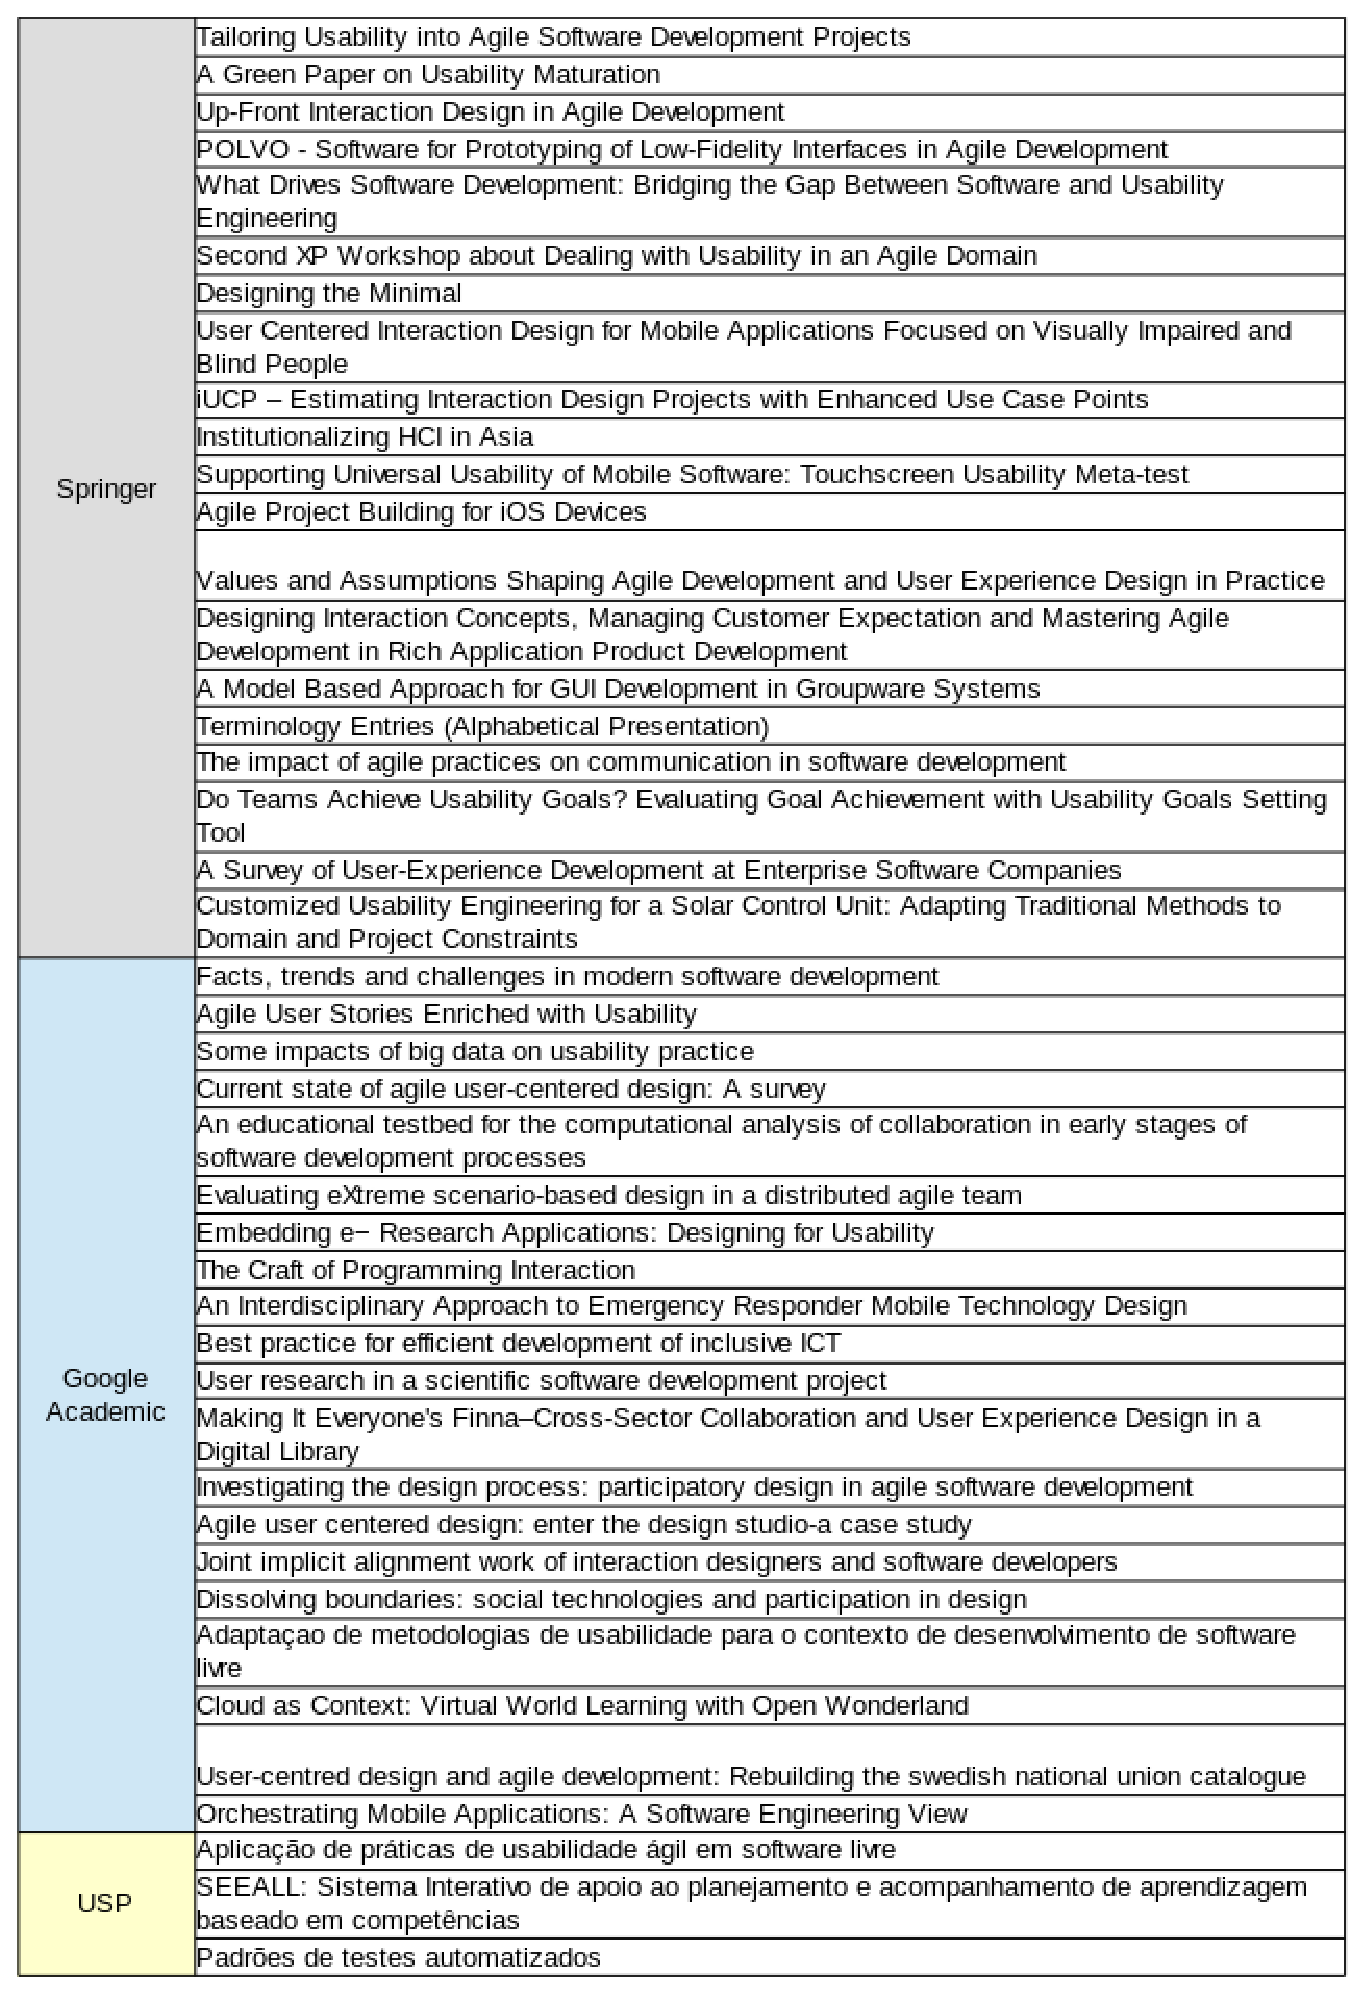
\includegraphics[width=1\textwidth]{figure/tabela1.eps}
    \caption{Resultado segunda etapa de seleção das publicações}
    \label{fig:tabela1}
  \end{center}
\end{figure}

%
Na terceira etapa de seleção das publicações, o resumo (abstract) de cada publicação foi lido. Seguindo o critério de seleção CS2, as publicações que não apresentavam o resumo (abstract) via engenho de busca foram descartadas automaticamente, assim selecionando dez publicações conforme apresentado na Figura \ref{fig:tabela2}.

\begin{figure}[hbt]
  \begin{center}
    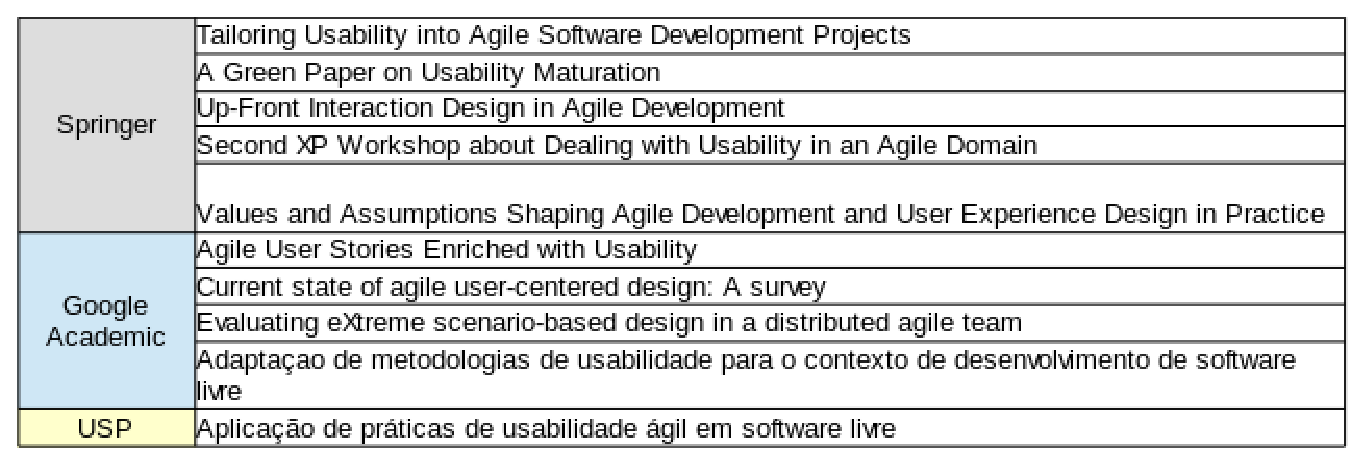
\includegraphics[width=1\textwidth]{figure/tabela2.eps}
    \caption{Terceira etapa de seleção das publicações}
    \label{fig:tabela2}
  \end{center}
\end{figure}

%
Na quarta etapa de seleção das publicações, foi realizada a leitura completa dos artigos aplicando o critério de seleção CS3 para verificar a adequação junto a hipótese levantada.

\subsection{Análise dos resultados da pesquisa}
Através da análise das técnicas encontradas é possível evidenciar as seguintes:

%
Aplicação do próprio processo de DCU (Design Centrado no Usuário) para levantamento dos usuários e do contexto de uso da metodologia. Os usuários do processo são membros de equipes de software livre, que desejam inserir práticas de usabilidade no processo de desenvolvimento. O contexto de uso são sistemas distribuídos geograficamente, com pessoas trabalhando colaborativamente. Os métodos podem ser aplicados tanto para o início de novos projetos, que tenham como usuários, pessoas não acostumadas a sistemas livres ou mesmo para a melhoria de sistemas existentes, com respeito à usabilidade.

%
Aplicação de definição de histórias de usuário de usabilidade dirigidas pela decisão do responsável por design realizando a prototipação dessas histórias e depois sendo validadas através de testes de usabilidade conforme figura abaixo.

%
As atividades de usabilidade seguem o modelo de ciclo de vida das outras atividades dentro do desenvolvimento ágil com a diferença que o ciclo de usabilidade tem sua iteração primeiro que as outras atividades de desenvolvimento conforme figura abaixo:

%
Aplicação das técnicas de usabilidade de acordo com as fases do DCU, conforme a descrição das técnicas de usabilidade das comunidades de métodos ágeis e de software livre. Para a fase do DCU Criar soluções de design, não foram identificadas propostas de adaptações, sendo portanto, descritas propostas para as fases: Identificar necessidades para design centrado em humano, Especificar contexto de uso, Especificar requisitos e Avaliar Designs conforme figura abaixo.

%
Algumas técnicas não muito aceitas pela comunidade de software livre devido a motivação partir de razões financeiras, mas exemplificadas:

%
Oferecimento de pagamento de US\$15,00 para pessoas que se interessem em testar a usabilidade de um sistema, o qual é fornecido por empresas que desejam obter um feedback sobre a usabilidade de seus projetos. Essa estratégia também difere das técnicas abordadas, pois os usuários envolvidos são motivados por razões financeiras e não filosóficas como no caso de sistemas livres e também por ser mais focada em avaliações de usabilidade e não em desenvolvimento com usabilidade.
%%----------------------------------------------------------------------------%%
\section{Considerações finais}
\label{sec:con_final}

O levantamento de técnicas de usabilidade da comunidade de métodos ágeis, técnicas de usabilidade ágil, e das técnicas de usabilidade da comunidade de software livre, foi realizado com o objetivo de refletir como técnicas de usabilidade poderiam ser aplicadas em comunidades de software livre.

%
Projetos de grande porte que geralmente possuem o patrocínio de grandes empresas, trás é melhor observado a aplicação das técnicas de usabilidade, pois estas podem contar com uma equipe formada por engenheiros de usabilidade e/ou especialistas em usabilidade. Já em projetos menores, raramente alguma prática de usabilidade é utilizada. Contudo, a maioria dos projetos de software livre e de projetos utilizando a metodologia ágil são desenvolvidos por equipes pequenas, compostas geralmente, apenas por desenvolvedores e que não possuem especialistas em usabilidade ou áreas relacionadas como participantes do projeto. Ainda assim, a usabilidade é importante neste contexto.

%
Algumas técnicas de usabilidade identificadas podem ser aplicadas sem nenhuma modificação em ambientes de desenvolvimento de software utilizando metodologia ágil, onde seja possível a realização de práticas presencialmente. Porém mesmo em um desenvolvimento distribuído é possível a aplicação dessas técnicas sem grandes modificações com apoio de ferramentas de comunicação via internet.

%
As técnicas foram retiradas de publicações que traziam a aplicação de técnicas de usabilidade dentro do ambiente de desenvolvimento ágil ocasionando o menor impacto possível nesse ambiente, o que facilita a compreensão e utilização dessas técnicas por parte de quase qualquer equipe de desenvolvimento ágil.

\bibliographystyle{sbc}
\bibliography{myReferences}
\end{document}
% vim: ts=2 sw=2 expandtab
